\documentclass{article}
\usepackage[UTF8, heading = false, scheme = plain]{ctex}

\usepackage{geometry}
\geometry{b5paper,left=2cm,right=2cm,top=2cm,bottom=2cm}

\usepackage{color}
\usepackage{amsfonts}
\usepackage{amsmath}

\linespread{1.5}
\usepackage{graphicx}

\usepackage[colorlinks,
            linkcolor=red,
            anchorcolor=blue,
            citecolor=green
            ]{hyperref}

\usepackage{listings}
\usepackage{fontspec}
\newfontfamily\monaco{Monaco}
\definecolor{dkgreen}{rgb}{0,0.6,0}
\definecolor{gray}{rgb}{0.5,0.5,0.5}
\definecolor{mauve}{rgb}{0.58,0,0.82}
\lstset{ %
  basicstyle=\footnotesize\monaco,       % the size of the fonts that are used for the code
  numbers=left,                   % where to put the line-numbers
  numberstyle=\footnotesize\monaco\color{gray},  % the style that is used for the line-numbers
  numbersep=5pt
  stepnumber=1,                   % the step between two line-numbers. If it's 1, each line
                                  % will be numbered
  numbersep=5pt,                  % how far the line-numbers are from the code
  backgroundcolor=\color{white},      % choose the background color. You must add \usepackage{color}
  showspaces=false,               % show spaces adding particular underscores
  showstringspaces=false,         % underline spaces within strings
  showtabs=false,                 % show tabs within strings adding particular underscores
  frame=single,                   % adds a frame around the code
  rulecolor=\color{black},        % if not set, the frame-color may be changed on line-breaks within not-black text (e.g. commens (green here))
  tabsize=4,                      % sets default tabsize to 2 spaces
  captionpos=t,                   % sets the caption-position to bottom
  breaklines=true,                % sets automatic line breaking
  breakatwhitespace=false,        % sets if automatic breaks should only happen at whitespace
  title=\lstname,                   % show the filename of files included with \lstinputlisting;
                                  % also try caption instead of title
  keywordstyle=\color{blue},          % keyword style
  commentstyle=\color{dkgreen},       % comment style
  stringstyle=\color{mauve},         % string literal style
  escapeinside={\%*}{*)},            % if you want to add LaTeX within your code
  morekeywords={*,...}               % if you want to add more keywords to the set
}

\usepackage{amssymb} 

\setlength{\parindent}{2em}

\renewcommand{\G}{\mathbb{G}}
\newcommand{\Z}{\mathbb{Z}}
\newcommand{\Q}{\mathbb{Q}}
\newcommand{\F}{\mathbb{F}}

\newcommand{\Sbox}{\textsf{Sbox}}
\newcommand{\code}[1]{\lstinline!#1!}

%%%%%%%处理下划线:_%%%%%%%%%
\usepackage{underscore}
%%%%%%%处理下划线:_%%%%%%%%%

\setlength{\parindent}{2.1em}

\begin{document}

\title{ Acceleraton of ECDSA Verification with Endomorphism Mapping of  secp256k1}
\author{longcpp \\ \small{longcpp9@gmail.com}}

\maketitle

Due to the fact that the ECDSA signature mechanism has been adopted by Bitcoin, 
the ECDSA signature mechanism based on the secp256k1 elliptic curve is widely used in the blockchain industry. 
At the very beginning, Bitcoin adopted the ECDSA signature mechanism based on secp256k1 implemented in OpenSSL,
where there is no targeted optimization for the secp256k1 curve 
leading to the low efficiency of the ECDSA based on the secp256k1 curve in OpenSSL. 
It is worth noting that the ESDSA signature mechanism based on the secp256r1 curve is deeply optimized in the OpenSSL project. The performance of these two ECDSAs in OpenSSL in running speed tests is given in Listing~\ref{openssl-bench}.

\lstinputlisting[firstline=9, lastline=72, caption=\texttt{openssl_ecdsa_benchmark},label=openssl-bench]{./openssl-bench.cpp}

The result of compiling and linking OpenSSL version 1.1 on the Intel(R) Core(TM) i7-6700HQ CPU shows that 
the running speed of the secp256k1-based ECDSA provided by OpenSSL is approximately 2000 sign/s and 2300 verify/s, 
while the running speed of ECDSA based on secp256r1 is about 33000 sign/s and 12000veriy/s. 
It can be said that the implementation speed of ECDSA based on the secp256k1 curve in OpenSSL 
is slower than that of the ECDSA based on the secp256r1 curve, by one order of magnitude. 
When it comes to security, according to the conclusion in \cite{ecdsa-side-channel}, 
the implementation of the secp256k1-based ECDSA in OpenSSL 1.1 is not secure.

The efficiency and security issues of OpenSSL implementation and the inconsistencies that 
may be introduced by OpenSSL version variations (See DER Encoding Rules and BIP 66) mean that 
it cannot meet the speed, security, and stability requirements of blockchain use cases. 
Bitcoin core developers of Bitcoin reimplemented the ECDSA based on secp256k1 in the libsep256k1 project, 
where the secp256k1 curve was deeply optimized and the constant implementation was guaranteed. 
Most blockchain projects adopting the ECDSA mechanism based on secp256k1 are currently using the implementation in libsec256k1 by default.

A great number of techniques are used in the libsep256k1 project to improve the efficiency of signature verification. 
We here only focus on the utilization of the endomorphism feature of secp256k1 to improve the efficiency of the verification. 
Prior to any technical discussions, we firstly show the speed improvements brought  by 
the endomorphism feature of secp256k1 in the libsecp256k1 project. 
It should be noted that in order to use the endomorphism feature to speed up the verification process, 
the \code{−−enable−endomorphism} option should be specified at the time of \code{./configure}; 
in order to use the built-in speed test cases of libsec256k1, \code{−enable−benchmark} should also be specified. 
When compiling without the  \code{−−enable−endomorphism} option, 
the results that come from the built-in test tool of libsecp256k1 are as follows:

\begin{lstlisting}[caption=\texttt{libsecp256k1 benchmark without --enable-endomorphism}]
$  secp256k1 git:(master) ./bench_sign
ecdsa_sign: min 45.6us / avg 46.1us / max 48.3us
$  secp256k1 git:(master) ./bench_verify 
ecdsa_verify: min 65.4us / avg 66.5us / max 68.6us
ecdsa_verify_openssl: min 471us / avg 474us / max 476us
\end{lstlisting}

Compiling with the \code{−−enable−endomorphism} option specified, 
the results that come from the built-in test tool of libsecp256k1 are as follows:

\begin{lstlisting}[caption=\texttt{libsecp256k1 benchmark with --enable-endomorphism}]
$  secp256k1 git:(master) ./bench_sign  
ecdsa_sign: min 45.5us / avg 46.1us / max 48.2us
$  secp256k1 git:(master) ./bench_verify 
ecdsa_verify: min 47.0us / avg 47.6us / max 49.6us
ecdsa_verify_openssl: min 470us / avg 476us / max 490us
\end{lstlisting}

As can be seen, whether the option of  \code{−−enable−endomorphism} option is speficied has no effect on the ECDSA signature speed. 
Each sign operation takes about 46 us, which is ~22000 sign/s. 
Specifiying the  \code{−−enable−endomorphism} option brings about a significantly increased speed of signature verification, 
from ~66.5 us to ~47.6 us, which is an increase from 15000 verify/s to 21000 verify/s (a speed improvement around 40\%). 
It is worth noting that the speed test tool of libsecp256k1 also tested the speed of secp256k1-based ECDSA in OpenSSL. 
The speed was around 475 us per verification, which was equivalent to 2100 verify/s. 
It is basically the same as the result of our previous test.  The results of all the above tests are given in Table~\ref{tbl-ecdsa-bench}. 
We will focus on the internals of the endomorphism feature in the next section.

\begin{table}[h]
\centering
\caption{ECDSA Speed Comparision}\label{tbl-ecdsa-bench}
\begin{tabular}{|c|c|c|c|c|c|}
\hline
\small
         & OpenSSL & OpenSSL & libsecp256k1 & libsecp256k1 \\
         & secp256r1 & secp256k1 & secp256k1  & secp256k1 \\
         &                 &                 & w.o. endomorphism & w. endomorphism \\\hline
 sign  & 33000/s  & 2000/s & 22000/s & 22000/s \\\hline
 verify & 12000/s & 2300/s & 15000/s & 21000/s \\\hline
\end{tabular}
\end{table}

As early as 2011, Bitcoin developer Hal Finney pointed out on Bitcointalk that 
the endomorphism feature of secp256k1 could be used to accelerate the signature verification of the ECDSA~\cite{halfinney}, 
Finney also gave the PoC code backing up the statement.
It can be seen by browsing the code implementation of libsecp256k1 that, 
the implementation in libsecp256k1 is based on the sample code given by Hal Finney, 
and the Hal Finney example is based on the content in Section 3.5 of \cite{guidetoecc}, 
which is basically a reproduce of contents from \cite{glv01}.

Assume $E$ is an elliptic curve defined over field $K$, we also use $E$ to denote the set of all points on this curve,
then  the endomorphism mapping in $E$ is a rational mapping $\phi: E \rightarrow E$ satisfying 
$$\phi(\mathcal{O}) = \mathcal{O}, \phi(P) = (g(P), h(P)), \forall P \in E,$$
where $g$ and $h$ are rational functions with coefficients  are elements of field $K$.
If $\phi_1$ and $\phi_2$ both endomorphisms of $E$, 
define the sum $\phi_1+\phi_2$  as $(\phi_1+\phi_2)(P) = \phi_1(P) + \phi_2(P)$,
and define the product of $\phi_1\phi_2$ as  $(\phi_1\phi_2)(P)=\phi_1(\phi_2(P))$,
then all endomorphisms of $E$ form a ring, called the endomorphism ring of $E$ over $K$.
Note that an endomorphism mapping $\phi$ is also a group homomorphism such that  
$$\phi(P_1 + P_2) = \phi(P_1) + \phi(P_2), \forall P_1, P_2 \in E.$$
 
Let $p\equiv 1 \mod 3$ be a prime and $E$ be an elliptic curve defined over $\F_p$ by $y^2 = x^3 + b$.
If $\beta\in\F_p$ is an element of order 3, then the following mapping is an endomorphism of $E$,
$$\phi(x,y) \rightarrow (\beta x, y), \phi(\mathcal{O}) = \mathcal{O}.$$
One can see that $\phi$ is truly a mapping from $E$ to $E$ by 
substituting $(\beta x, y)$ into the equation of $E$: $y^2 = (\beta x)^3 + b = \beta^3x^3 + b$.
As $order(\beta)=3$ ($\beta^3 \equiv 1 \mod p$), we have $y^2 = (\beta x)^3 + b = \beta^3x^3 + b  = x^3 + b$.
The characteristic polynomial of the endomorphism $\phi: E \rightarrow E$ is $X^2 + X + 1$.
Then characteristic polynomial of an endomorphism is the monic polynomial $f(X)$ of least degree in $\Z[X]$
such that $f(\phi)(P)=\mathcal{O}, \forall P\in E$. 
We can verify that endomorphism $\phi$ truly satisfies $f(\phi)(P)=\mathcal{O}, \forall P\in E$, i.e.
$$(\phi^2+\phi+1)(P) = \mathcal{O}, \forall P \in E.$$
Denote $P\in E$ as $(x,y)$, according to the definition of the endomorphism mapping $\phi$ we have 
$$(\phi^2+\phi+1)(P) = \phi^2(P) + \phi(P) +1(P) = (\beta^2 x, y) + (\beta x, y) + (x,y).$$
By the definition of point addition formula given by \cite{Blahut14} as in Figure~\ref{fig-ecpoint-add}, one get 
 $$(\beta^2 x, y) + (\beta x, y) + (x,y) = (-\beta^2 x -\beta x, -y) + (x,y).$$
 As $\beta^3 \equiv 1 \mod p$, then $\beta^2+\beta+1=0$, thus
 $$ (-\beta^2 x -\beta x, -y) + (x,y) = (-(\beta^2+\beta) x, -y) = (x,-y) + (x,y) = \mathcal{O}.$$


\begin{figure}
\centering
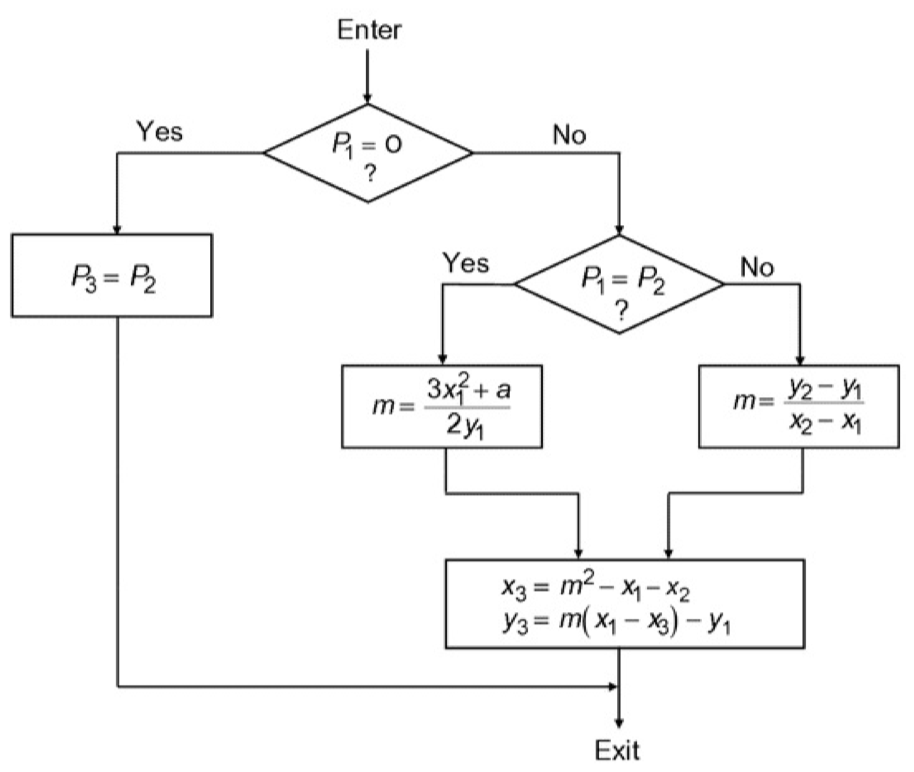
\includegraphics[width=.7\textwidth]{ec-point-addition.png}
\caption{Point addtiion of $E: y^2=x^3+b$, i.e. $(x_3,y_3)=P_3=P_1+P_2=(x_1,y_1) + (x_2,y_2)$}\label{fig-ecpoint-add}
\end{figure}

Suppose $E$ is an elliptic curve defined over the finite field $\F_p$ with $p$ being a large prime number s.t. $p \equiv 1 \mod 3$,
denote the number of elements of $E(\F_p)$ with $\#E(\F_p)$, and the largest prime factor of $\#E(\F_p)$ s.t. $n^2 \nmid \#E(\F_p)$,
then point group $E(\F_p)$ contains exactly one subgroup of order $n$.
Denote the base point (generator) of this subgroup with $G\in E(\F_p)$, and denote the subgroup as $\G = \langle G \rangle$,
then the aforementioned mapping $\phi$ acts on $\G$ (assuming $\phi(G)\neq \mathcal{O}$) as a multiplication mapping: 
$$\phi(G) = \lambda G, \lambda^2 + \lambda + 1 \equiv 0 \mod n.$$

Elliptic curve secp256k1 $y^2 = x^3 + 7$ is defined over finite field $\F_p$ where
\small
$$p = 0xfffffffffffffffffffffffffffffffffffffffffffffffffffffffefffffc2f.$$
\normalsize
$\#E(\F_p) = h \cdot n$ with cofactor $h = 1$ and $n$ being the order of largest subgroup of $E(\F_p)$:
\small
$$ n = 0xfffffffffffffffffffffffffffffffebaaedce6af48a03bbfd25e8cd0364141.$$
\normalsize
Base point $G$ of subgroup of $\G = \langle G \rangle$ is 
$$G_x = 0x79be667ef9dcbbac55a06295ce870b07029bfcdb2dce28d959f2815b16f81798$$
$$G_y = 0x483ada7726a3c4655da4fbfc0e1108a8fd17b448a68554199c47d08ffb10d4b8$$
Note that the parameters $p\equiv 1 \mod 3, n | \#E(\F_p), n^2 \nmid \#E(\F_p)$,
then exists $\phi$ s.t. 
$$
\phi(P) = \phi(x, y) = (\beta x, y) = \lambda P, \beta^3 \equiv 1 \mod p, \lambda^2 + \lambda + 1 \equiv 0 \mod n, \forall P \in \G.
$$
Note that 
$$\lambda P = (\beta x, y) \rightarrow \lambda^2 P = (\beta^2 x, y) \rightarrow \lambda^3 P = (\beta^3 x, y) = (x, y),$$
then $\lambda^3 \equiv 1 \mod n$ ($\lambda^2+\lambda + 1 \equiv 0 \mod n$).
The value of $\beta, \lambda$ can be computed via Fermat's Little Theorem as in Listing~\ref{lst-betalamb}.

\begin{lstlisting}[language=python, caption=\texttt{generate $\beta$ and $\lambda$ for endomorphism of secp256k1}, label=lst-betalamb]
sage: p = 0xfffffffffffffffffffffffffffffffffffffffffffffffffffffffefffffc2f
sage: n = 0xfffffffffffffffffffffffffffffffebaaedce6af48a03bbfd25e8cd0364141
sage: fp = GF(p)
sage: fn = GF(n)
sage: beta = fp(2)^((fp.characteristic()-1)/3)
sage: lamb = fn(3)^((fn.characteristic()-1)/3)
sage: hex(int(beta))
'0x7ae96a2b657c07106e64479eac3434e99cf0497512f58995c1396c28719501eeL'
sage: hex(int(lamb))
'0x5363ad4cc05c30e0a5261c028812645a122e22ea20816678df02967c1b23bd72L'
\end{lstlisting}

With the specific values of $\beta, \lambda$ and the parameters of secp256k1, we can verify aforementioned theory, 
e.g. $(\phi^2+\phi + 1)(P) = \mathcal{O}$,  $\lambda P = (\beta x, y)$, refer to Listing~\ref{lst-verifyphi}.

\begin{lstlisting}[language=python, caption=\texttt{verify endomorphism $\phi$ with $\beta, \lambda$ for secp256k1}, label=lst-verifyphi]
sage: secp256k1 = EllipticCurve(fp, [0,7])
sage: P = secp256k1.random_point()
sage: beta_P = int(lamb) * P
sage: beta2_P = int(lamb * lamb) * P
sage: secp256k1.is_on_curve(P.xy()[0], P.xy()[1])
True
sage: secp256k1.is_on_curve(beta_P.xy()[0], beta_P.xy()[1])
True
sage: secp256k1.is_on_curve(beta2_P.xy()[0], beta2_P.xy()[1])
True
sage: P + beta_P + beta2_P
(0 : 1 : 0)
sage: P
(41377969691400010933106372906063172361899533199914561951528196380352494104025 : 
98022602531930804648533646821930292808872917654793309549219646753654843391634 : 1)
sage: beta_P
(61065808270983873313809816182282167124533426070191311711991257449293116444501 : 
98022602531930804648533646821930292808872917654793309549219646753654843391634 : 1)
sage: beta2_P
(13348311274932311176654795920342568366837025395534690375938130178263224123137 : 
98022602531930804648533646821930292808872917654793309549219646753654843391634 : 1)
sage: beta * P.xy()[0]
61065808270983873313809816182282167124533426070191311711991257449293116444501
sage: beta * beta * P.xy()[0]
13348311274932311176654795920342568366837025395534690375938130178263224123137
\end{lstlisting}

Endomorphism mapping of secp256k1 can be used to speed up point multiplication, and thus ECDSA verification speed can be improved.
Refer to Figure~\ref{fig-ecdsa} from \cite{stallings}, one can see  that 
only fixed point multiplication is involved in ECDSA signing procedure.
Fixed-point multiplication can be effectively calculated by using pre-calculation and 
hence there no need to utilize endomorphism mapping for ECDSA signing procedure
\footnote{Need to further verify this statement. Intuitively, fixed point multiplication via precomputed table 
would be faster than utilizing the endomorphism mapping}.
However, during the verification procedure, one need to compute $es^{-1}G+rs^{-1}Q$, 
where $r,s$ is the signature value and $e$ is the integer converted from the hash value of the message to be signed.
The computation of $rs^{-1}Q$ can be improved with endomorphism mapping.
In the next section, we will discuss how to use the endomorphism $\phi$ to accelerate the multiplication of non-fixed points, 
thus improving the efficiency of ECDSA’s signature verification procedure. 

\begin{figure}[h]
\centering
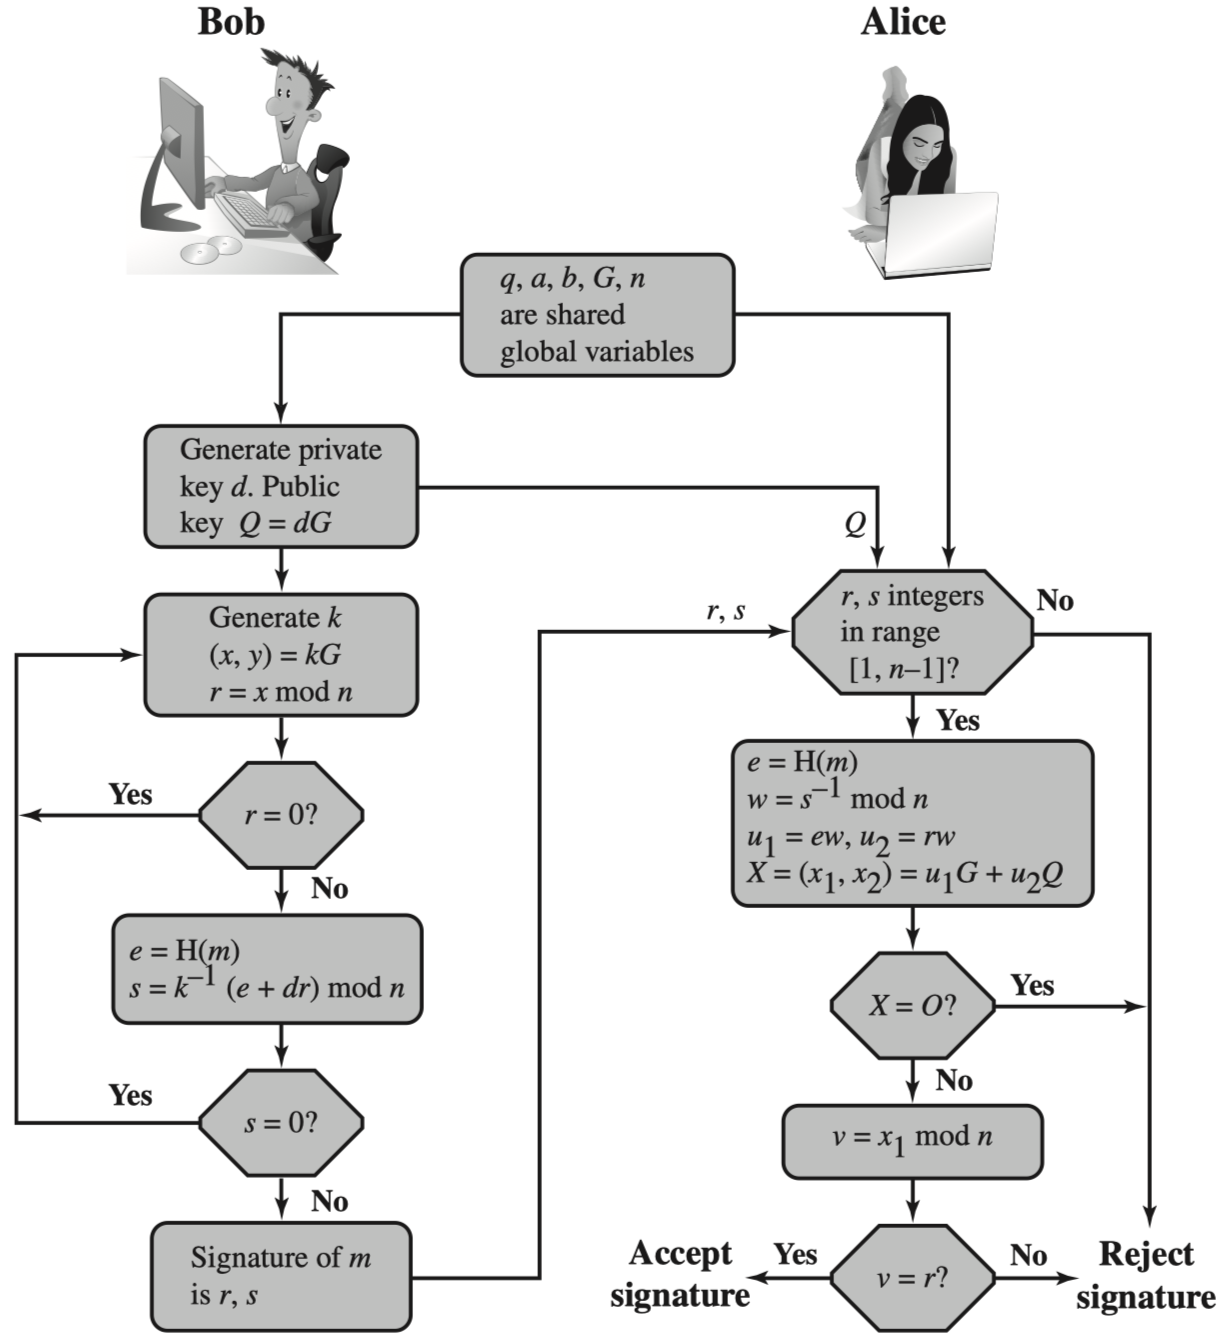
\includegraphics[width=.8\textwidth]{ecdsa.png}
\caption{ECDSA签名验签}\label{fig-ecdsa}
\end{figure}

Denote the point multiplication to be computed is $kP$,
we need to represent $k$ as $k=k_1+k_2\lambda \mod n$, 
where the bits' length of $k_1, k_2$ are roughly half of $k$'s, then we have
$$kP = k_1P + k_2\lambda P = k_1P + k_2\phi(P) = k_1 P + k_2 Q, Q = \phi(P),$$
where the computation of $Q=\phi(P)$ requires only one field multiplication as $(x_Q, y_Q) = (\beta x_P, y_P)$,
and $k_1 P + k_2 Q$ can be efficiently computed via simultaneous multiple point multiplication.

Decomposition of $k = k_1+k_2\lambda \mod n$ is discussed in \cite{glv01}, 
the complete algorithm is given in \cite{guidetoecc} as Algorithm 3.74.
The algorithm takes in $n, \lambda, k\in [1, n-1]$ and output $(k_1, k_2) \in \Z \times \Z$ s.t.  
$k \equiv k_1 + k_2 \lambda \mod n$ and the Euclidean Norm of $(k_1, k_2)$ is relatively small.
Define homorphic mapping $f: \Z\times\Z \rightarrow \Z_n$ as $(i,j) \rightarrow i + j\lambda$,
what we are trying to find is a vector $\mathbf{k}=(k_1, k_2)\in \Z\times\Z$ satisfying $f(\mathbf{k})= k$.
Note that $\mathbf{k} = (k, 0)$ satisfies the aforementioned conditions, but is not useful to our purpose.
What we need is a vector $\mathbf{k}$ with relatively small Euclidean norm.

The method given in ~\cite{glv01} is to firstly find two linearly independent vectors $\mathbf{v_1}, \mathbf{v_2} \in \Z \times \Z$,
s.t. $f(\mathbf{v_1}) = f(\mathbf{v_2}) = 0$, then find a vector  generated by $\mathbf{v_1}, \mathbf{v_2}$: 
$\mathbf{v} = \beta_1\mathbf{v_1} + \beta_2\mathbf{v_2}$  close to vector $(k,0)$. 
Then $\mathbf{k} = (k,0) - \mathbf{v}$ is a short vector satisfying $f(\mathbf{k}) = f((k,0)) - f(\mathbf{v}) = k$.

We can use the Extended Euclidean Algorithm to find vectors $\mathbf{v_1}$ and $\mathbf{v_2}$.
When applying the Extended Euclidean Algorithm $n$ and $\lambda$,
a series of equations will be produced:
\begin{equation}
\label{eq-eea}
s_i n. + t_i \lambda = r_i, i = 0, 1, 2, ....
\end{equation}
where $s_0 = 1, t_0 = 0, r_0 = n, s_1 =0, t_1 = 1, r_1 = \lambda$ and $r_i \ge 0$.
Then we have the following properties:
\begin{enumerate}
\item $r_i > r_{i+1} \ge 0 \text{ for all } i \ge 0$
\item $|s_i| < |s_{i+1}| \text{ for all } i \ge 1$
\item $|t_i| < |t_{i+1}| \text{ for all } i \ge 0$
\item $r_{i-1}|t_i| + r_i|t_{i-1}| = n \text{ for all } i \ge 1$
\end{enumerate}
The 2nd and 3rd properties can be  proved according to the computation of $s_i$ and $t_i$:
\begin{equation}\nonumber
s_i = \left\{
\begin{array}{ll}
1 & \text{ if } i = 0 \\
0 & \text{ if } i = 1, \\
s_{i-2} - q_{i-1}s_{i-1} & \text{ if } i \ge 2 
\end{array}
\right. 
t_i = \left\{
\begin{array}{ll}
0 & \text{ if } i = 0 \\
1 & \text{ if } i = 1 \\
t_{i-2} - q_{i-1}t_{i-1} & \text{ if } i \ge 2 
\end{array}
\right.
\end{equation}
As $s_2 = 1$ and $s_3$ is negative, then $s_4 = s_2 - q_3s_3$ is positive, 
then the following  $s_{i}$ alternate in sign and strictly increase in magnitude, 
Thus $|s_i| < |s_{i+1}| \text{ for all } i \ge 1$.
Similarly, $|t_i| < |t_{i+1}| \text{ for all } i \ge 0$ can be proved.
The 4th property can be proved inductively.
Suppose when $i = 1$, equation $r_0|t_1| + r_1|t_0| = n \cdot 1 + \lambda \cdot 0 = n$ holds.
We then further assume that $r_{i-1}|t_i| + r_i|t_{i-1}| = n$ holds, consider $r_{i}|t_{i+1}| + r_{i+1}|t_{i}|$:
\begin{equation}\nonumber
\begin{split}
r_{i}|t_{i+1}| + r_{i+1}|t_{i}| = & r_{i}|t_{i-1} - q_{i}t_{i}| + (r_{i-1}-q_{i}r_{i})|t_{i}| \\
= & r_i|t_{i-1}| + r_iq_i|t_i| + r_{i-1}|t_i| - q_ir_i|t_i|\\
= & r_i|t_{i-1}|+ r_{i-1}|t_i| = n.
\end{split}
\end{equation}
We use $m$ to denote the biggest $m$ s.t. $r_m \ge \sqrt{n}$,
the according to the 4th property, we have $r_m|t_{m+1}| + r_{m+1}|t_m| = n$, and hence $|t_{m+1}|<\sqrt{n}$.
According to Equaiton (\ref{eq-eea}), we have
$$s_{m+1}n + t_{m+1}\lambda = r_{m+1} \rightarrow r_{m+1} - t_{m+1} \lambda = s_{m+1} n \equiv 0 \mod n.$$
Let $(a_1, b_1) = \mathbf{v_1}  = (r_{m+1}, - t_{m+1})$, then $f(\mathbf{v_1}) = 0$ is satisfied.
As $|t_{m+1}|<\sqrt{n}$ and $|r_{m+1}| < \sqrt{n}$,  then the Euclidean norm of $\mathbf{v_1}$ satisfy $||\mathbf{v_1}|| <\sqrt{2n}$.
Let $(a_2, b_2) = \mathbf{v_2}$ be one of $(r_{m}, - t_{m})$和$(r_{m+2}, - t_{m+2})$ with the smaller Euclidean norm,
then according to Equaiton (\ref{eq-eea}), $f(\mathbf{v_2}) = 0$.
Heuristically, $\mathbf{v_2}$ is also short.
Note that $\mathbf{v_1}$ and $\mathbf{v_2}$ are linearly indepenndent. 
Otherwise, w.o.l.g.  by assuming $\mathbf{v_2}=(r_m,-t_m)$, we have
$$
\dfrac{r_{m+1}}{r_m} = \dfrac{-t_{m+1}}{-t_m} = \dfrac{t_{m+1}}{t_m},
$$
As $\frac{r_{m+1}}{r_m} < 1$ and $|\frac{t_{m+1}}{t_m}| > 1$, resulting in contradiction.

With the value of $\mathbf{v_1}$和$\mathbf{v_2}$, we try to build vector 
$\mathbf{v} = \beta_1\mathbf{v_1} + \beta_2\mathbf{v_2}$ that is close to $(k,0)$.
As there might be no $\beta_1, \beta_2 \in \Z$ such that $\mathbf{v} = \beta_1\mathbf{v_1} + \beta_2\mathbf{v_2}$ holds,
thus we consider in $\Q\times\Q$, e.g. $\beta_1, \beta_2 \in \Q$.
After obtain $\beta_1, \beta_2 \in Q$, we then round $\beta_1, \beta_2$ to the nearest integers in $\Z$ as $c_1, c_2$,
and denote $\mathbf{v} = c_1\mathbf{v_1} + c_2\mathbf{v_2}$, then the vector we are trying to find is 
$$\mathbf{k} = (k,0) - \mathbf{v} = (k, 0) - c_1\mathbf{v_1} + c_2\mathbf{v_2},$$
where $k_1 =  k - c_1a_1 - c_2a_2, \ k_2 = \ -c_1b_1-c_2b_2$.

\begin{figure}[h]
\centering
\caption{Algorithm 3.74: Decompose $k$ in \cite{guidetoecc}~}\label{fig-splitk}
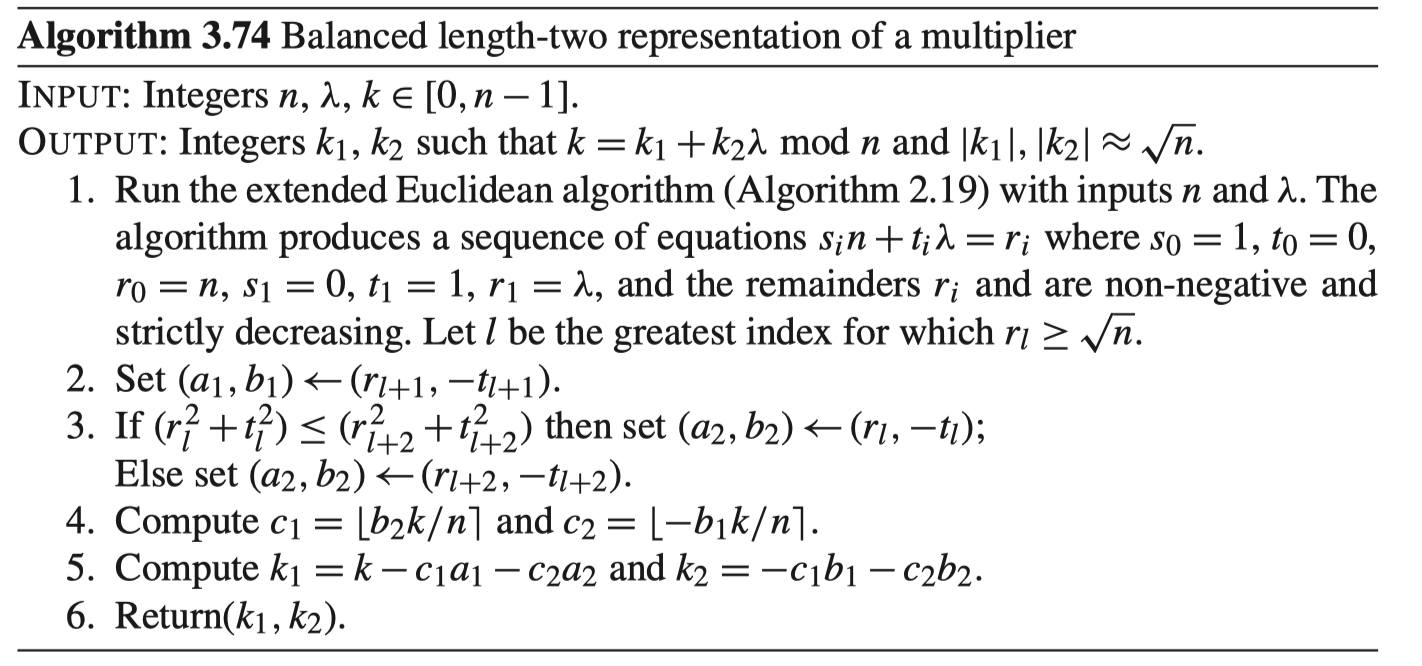
\includegraphics[width=\textwidth]{split-k.png}
\end{figure}

Now we discuss how to compute $\beta_1, \beta_2$. As $(k, 0) = \beta_1(a_1,b_1) + \beta_2(a_2, b_2)$, then
\begin{equation}\nonumber
\begin{split}
\beta_1a_1 + \beta_2a_2 =& \  k\\
\beta_1b_1 + \beta_2b_2 =& \ 0
\end{split}
\end{equation}
By solving the equation group, we get
$$
\beta_1 = \dfrac{b_2k}{a_1b_2 - a_2b_1}, \ \beta_2 = \dfrac{-b_1k}{a_1b_2-a_2b_1}.
$$
As $(a_1, b_1) = (r_{m+1}, - t_{m+1})$ and  w.o.l.g. we assume $(a_2, b_2) = (r_{m}, - t_{m})$, 
According to the 4th property and the fact the two consecutive elements in series of $t_i$ have different signs, we have
$$|a_1b_2-a_2b_1| = |-r_{m+1}t_{m}+ t_{m+1}r_{m}| = n,$$
and hence
$$\beta_1 = b_2k / n, \ \beta_2 = -b_1k/n, \ c_1 = \lfloor \beta_1 \rceil, \  c_2 = \lfloor \beta_2 \rceil.$$
With the above discussion, we now have a better understanding of Algorithm 3.74, refer to Figure~\ref{fig-splitk}.

Implementation of Figure~\ref{fig-splitk} in Sage is give in Listing~\ref{lst-splitk}, where we also output the values of 
$a_1, b_1, a_2, b_2, c_1, c_2$ to verify the correctness of the implementation.
One can see that values of $a_1, b_1, a_2, b_2, c_1, c_2$ are the same as those given by Finney in \cite{halfinney}.

\lstinputlisting[caption=\texttt{split_k with $\lambda$ for secp256k1},label=lst-splitk]{./split-k.sage}

To further verity the correctness of the decomposition of $k$, in Listing~\ref{lst-splitkverify}
a randomly chosen $k$ is split into $k_1, k_2$, and verifies that $k_1 + k_2\lambda\equiv k\mod n$.
\begin{lstlisting}[language=python, caption=\texttt{verify multiplier split  with $\lambda$ for secp256k1}, label=lst-splitkverify]
sage: load("split-k.sage")
sage: k = int(fn.random_element())
sage: k1, k2 = split_k(n, int(lamb), k)
k 0x572d5beb0549d2ddcb1ff17bc516568c7f2a4d776e9c15d86e42ae55396f34f5L
a1, b1 0x3086d221a7d46bcde86c90e49284eb15L -0xe4437ed6010e88286f547fa90abfe4c3L
a2, b2 0x114ca50f7a8e2f3f657c1108d9d44cfd8L 0x3086d221a7d46bcde86c90e49284eb15L
c1, c2 0x10866a88d9692d0cb6a3e3188351f370L 0x4dbb61ed92bcc5654a28486a8793676aL
k1, k2 0x4cfc491368f8e9bb17180d76c4587555L 0x6bb2c62e9346d862c0edd4a2cf1e649eL
sage: (k1 + k2 * int(lamb)) % n
39431360339721158570738739562322678290810515502148100028669271620139548095733
sage: k
39431360339721158570738739562322678290810515502148100028669271620139548095733L
\end{lstlisting}

With the values of $a_1, b_1, a_2, b_2, c_1, c_2$, Finney gave the PoC code utilizing OpenSSL in~\cite{halfinney}.
Due to the evolvement of OpenSSL, we need to slightly modify Finney's code to successfully compile the code with OpenSSL 1.1.
The adjusted code is listed in Listing~\ref{lst-endpoc} and results show that by utilizing the endomorphism mapping 
the verification procedure is improved by \~16\%.

\lstinputlisting[firstline=67, lastline=155, firstnumber=67, caption=\texttt{PoC of speeding up ECDSA verification with endomorphism},label=lst-endpoc]{./secp256k1-endomorphism.c}

The \~40\% improvement in libsecp256k1 is achieved by utilizing more techniques, such as 
avoiding division operation when decomposing $k$ by precomputation, we will further investigate this in the future.

\begin{thebibliography}{99}

\bibitem{ecdsa-side-channel}
Genkin, Daniel, Lev Pachmanov, Itamar Pipman, Eran Tromer, and Yuval Yarom. "ECDSA key extraction from mobile devices via nonintrusive physical side channels." In Proceedings of the 2016 ACM SIGSAC Conference on Computer and Communications Security, pp. 1626-1638. ACM, 2016.

\bibitem{halfinney}
Hal Finney. bitcointalk - Speeding up signature verification. 2011.
\url{https://bitcointalk.org/index.php?topic=3238.0}

\bibitem{guidetoecc}
Hankerson, Darrel, Alfred J. Menezes, and Scott Vanstone. "Guide to elliptic curve cryptography." Computing Reviews 46, no. 1 (2005): 13.

\bibitem{Blahut14}
Blahut, Richard E. Cryptography and secure communication. Cambridge University Press, 2014.

\bibitem{stallings}
Stallings, William. Cryptography and network security: principles and practice. Upper Saddle River: Pearson, 2017.

\bibitem{glv01}
Gallant, Robert P., Robert J. Lambert, and Scott A. Vanstone. "Faster point multiplication on elliptic curves with efficient endomorphisms." In Annual International Cryptology Conference, pp. 190-200. Springer, Berlin, Heidelberg, 2001.

\end{thebibliography}

\end{document}